\chapter{Introducci\'{o}n y Objetivos}
\label{chap:intro}
\graphicspath{{intro/figs/}{intro/figs/}}

%******************************************************************************************************************************************************


Nos encontramos ante una autentica revolución en el sector de la ingeniería y las telecomunicaciones: la mejora y abaratamiento de las tecnologías y redes inalámbricas están cambiando la forma en la que interactuamos con nuestro entorno. Esto, unido a la aparición de nuevas tecnologías en el procesado de datos, ha propiciado una mayor demanda por parte de la industria.
\paragraph{}
El término \textit{IoT} (Internet of things) es un concepto que hace referencia a este fenómeno y que consiste en la conexión de elementos cotidianos a la red. A día de hoy, podemos encontrar desde bombillas hasta extensas redes de farolas interconectas.
\paragraph{}
Según datos del IDC (International Data Corporation), para 2019 se prevé que la inversión mundial en \textit{IoT} supere los \$745 mil millones de dolares, lo que supone un 15,4\% más que el año pasado. Se espera que el ritmo de crecimiento continue los próximos años llegando a superar \$1 billón de dólares en 2022.
\paragraph{}
Ante este panorama, se hace evidente la necesidad de innovar y desarrollar soluciones más eficientes. El creciente aumento en el número de dispositivos conectados hace necesario el desarrollo de redes y tecnologías más robustas, que soporten el gran volumen de datos actual y el esperado en años venideros.
\paragraph{}
En esta primera parte, expondré brevemente las tecnologías utilizadas actualmente en la industria así como sus ventajas e inconvenientes. Finalmente me centraré en la tecnología utilizada en este proyecto, las motivaciones para usarla y los objetivos que busco alcanzar en este TFG. 


\subsection{Tecnologías actuales }

En el mercado actual podemos encontrar un amplio abanico de tecnologías de comunicación inalámbrica. Aunque estas tecnologías  distan, en ocasiones, mucho unas de otras, podemos caracterizarlas y compararlas mediante tres factores fundamentales: potencia, alcance y ancho de banda. Estos factores tienen fuertes interdependencias entre si, lo que hace complicado cumplirlos todos a la vez. Esta problemática se ve reflejada en la figura \ref{fig:CVA}: si queremos dos de los factores tenemos que renunciar al tercero.

\begin{figure}[!h]
    \centering
    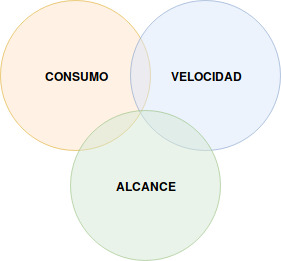
\includegraphics[width=0.3\linewidth]{CVA.jpg}
    \caption{Parámetros fundamentales de un sistema inalambrico}
    \label{fig:CVA}
\end{figure}
Algunas de las tecnologías usadas para \textit{IoT} son:

\begin{itemize}
    \item \textbf{NFC:} (Near Field Communication) es un estándar de comunicaciones de corto alcance inalámbricas desarrollado por Sony y NPX. Trabaja en la frecuencia de 13.56MHz utilizando modulaciones OOK (on-off keying) y BPSK. Esta tecnología alcanca velocidades de transmisión de hasta 848Kbps, dependiendo del entorno en el que se lleve acabo la comunicación. 
    
    Esta tecnología no requiere altas potencias en transmisión, pero no alcanza grandes tasas binarias y su alcance se limita a algunos centímetros.
    
    \item \textbf{WiFi: } Tecnología de comunicación de corto alcance inalámbrica que utiliza el estándar IEEE 802.11x. Utiliza las bandas ISM de 2.4 GHz y 5.7 GHz, utilizando un amplio número de modulaciones (varían según la banda y versión del estándar). Es uno de los estándares mas utilizados en la industria por su aplicación en redes locales (WLAN) y por las altas tasas binarias que alcanza (1.3 Gbps teóricos y hasta 400 Mbps reales).
    
    Este sistema requiere potencias mayores para su funcionamiento, su alcance esta limitado a algunas decenas de metros y su velocidad binaria está limitada por el entorno (el amplio número de redes que coexisten actualmente limitan su funcionamiento).
    
    \item \textbf{BLE:} (Bluetooth Low Energy) Se trata de una tecnología de comunicaciones de corto alcance, diseñada por Bluetooth Special Interest Group. Utiliza la banda ISM de 2.4 GHz y alcanza tasa binarias de hasta 1.37 Mbps. 
    Este sistema destaca por su bajo consumo, pero tiene un alcance limitado y una tasa binaria no muy alta. 
    
    \item \textbf{WiMAX:} (World Interoperability for Microwave Access) Es un tecnología basada en el estándar IEEE 802.16, la cual puede dar servicio a redes de area metropolitana. Utiliza las bandas entre 2.3 y 5.8 GHz y puede alcanzar tasas binarias de hasta 20 Mbps. Destaca por su amplio alcance (hasta 70 Km), pero requiere mucha potencia para su funcionamiento.


\end{itemize}

    
    A parte de estas, existen muchas otras tecnologías, cuyas características se resumen en en la figura \ref{fig:PWCA}
    
    \begin{figure}[!h]
        \centering
        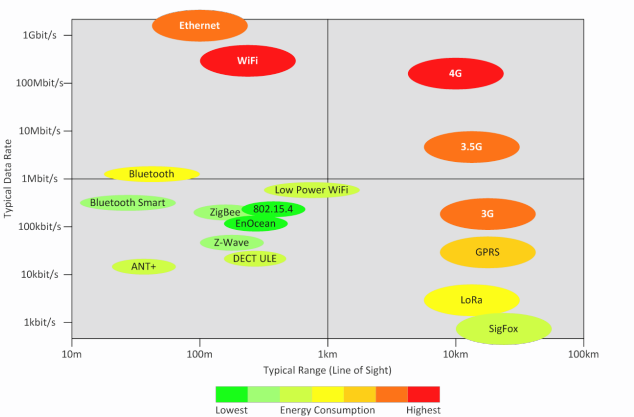
\includegraphics[width= 0.7\linewidth]{PWCVA.png}
        \caption{Relación consumo/velocidad/alcance de las diferentes tecnologías} 
        \label{fig:PWCA}
    \end{figure}
    
    
    \subsection{Redes LPWAN}
    
    Se definen como redes de bajo consumo y largo alcance (LPWAN de sus siglas en inglés), al conjunto de redes inalámbricas caracterizadas por tener largos alcances, consumo mínimo y baja tasa binaría. Su bajo consumo posibilita implementarlo sobre dispositivos alimentados mediante baterías.
    
    \paragraph{}
    
    Uno de los principales inconvenientes de estas tecnologías es su baja tasa binaria, la cual hace imposible la transmisión de grandes volúmenes de datos y a su vez limita su utilización a sistemas con interfaces máquina a máquina (M2M de sus siglas en inglés). Las tasas binarias con las que trabajan las redes LPWAN rondan los 0.3 Kbps y los 50 Kbps, dependiendo principalmente de las técnicas de transmisión y los estándares utilizados.  
    \paragraph{}

    Para conseguir estas características, las redes LPWAN utilizan diferentes técnicas como:
    \begin{itemize}
        \item \textbf{Ultra Narrowband (UNB): } Se traduce como "banda ultra-estrecha". Su funcionamiento se basa en la utilización de canales con poco ancho de banda para trasmitir.Su reducido ancho de banda conlleva menor consumo, un uso más eficiente del espectro y un aumento drástico del número de dispositivos que pueden operar en una misma red.
        
        
        \item \textbf{Spread Spectrum (SS):} Se trata de una modulación de espectro ensanchado en la cual, a cada canal, se le otorga un ancho de banda mayor al estrictamente necesario para funcionar. Al aumentar el ancho de banda, aumentamos la energía por bit utilizada, mejorando el ratio señal a ruido en el receptor. 
                
        
    \end{itemize}    
    
    \pagebreak
    
           \begin{figure}[!h]
            \centering
            
            \begin{subfigure}[t]{0.5\textwidth}
                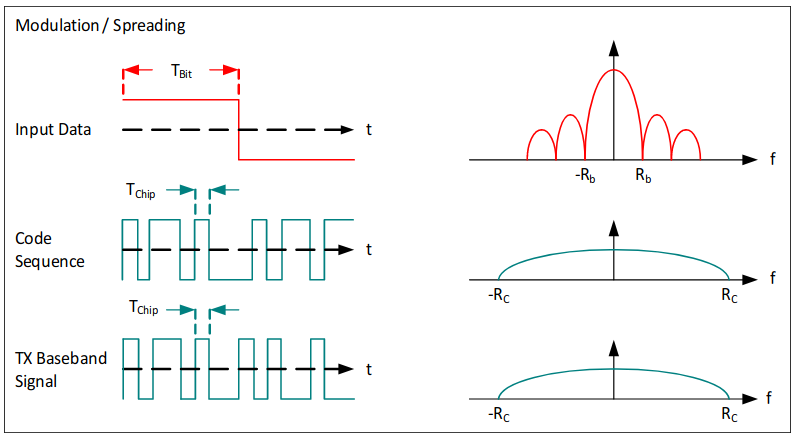
\includegraphics[width = \linewidth]{CSS.png}
                \caption{Modulación, ensanchado del espectro \citep{LoRaMod} }
                \label{fig:my_label}
            \end{subfigure}%
            \hfill
            \begin{subfigure}[t]{0.5\textwidth}
                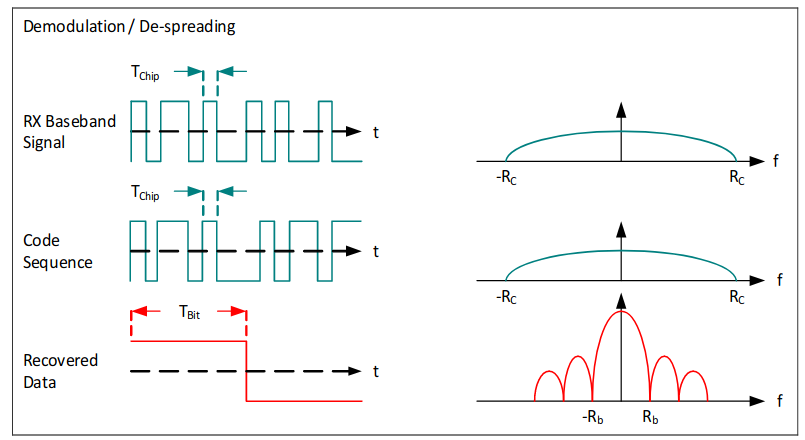
\includegraphics[width = \linewidth]{DeCSS.png}
                \caption{Caption}
                \label{fig:my_label}
            \end{subfigure}
            
            \begin{subfigure}[t]{0.5\textwidth}
    			\centering
    			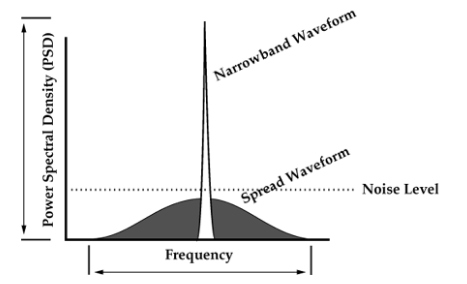
\includegraphics[width =\linewidth]{UNBvsSS.png}
    			\caption{Comparativa entre banda estrecha y espectro ensanchado}
    		\end{subfigure}

        \end{figure}
        

    
    \subsection{LoRa}
    
    LoRa (Long Rate) es una técnica de modulación  en espectro ensanchado, basada en la modulación Chirp de espectro ensanchado CSS (Chirp Spread Spectrum). LoRa es una modulación propietaria, desarrollada for la empresa francesa Cycle y posteriormente adquirida por Semtech Corporation.
    \paragraph{}
	La modulación Chirp de espectro ensanchado se basa en la utilización de pulsos chirp lineales para modular la señal. Un chirp es una señal sinusoidal cuya frecuencia varia con el tiempo. La utilización de chirps para modular la señal hace al sistema robusto frente al desvanecimiento debido al multitrayecto, ruido pulsante en banda estrecha e interferencias debidas al efecto doppler.
		
	\begin{figure}[h!]
            \begin{subfigure}[t]{0.5\textwidth}
                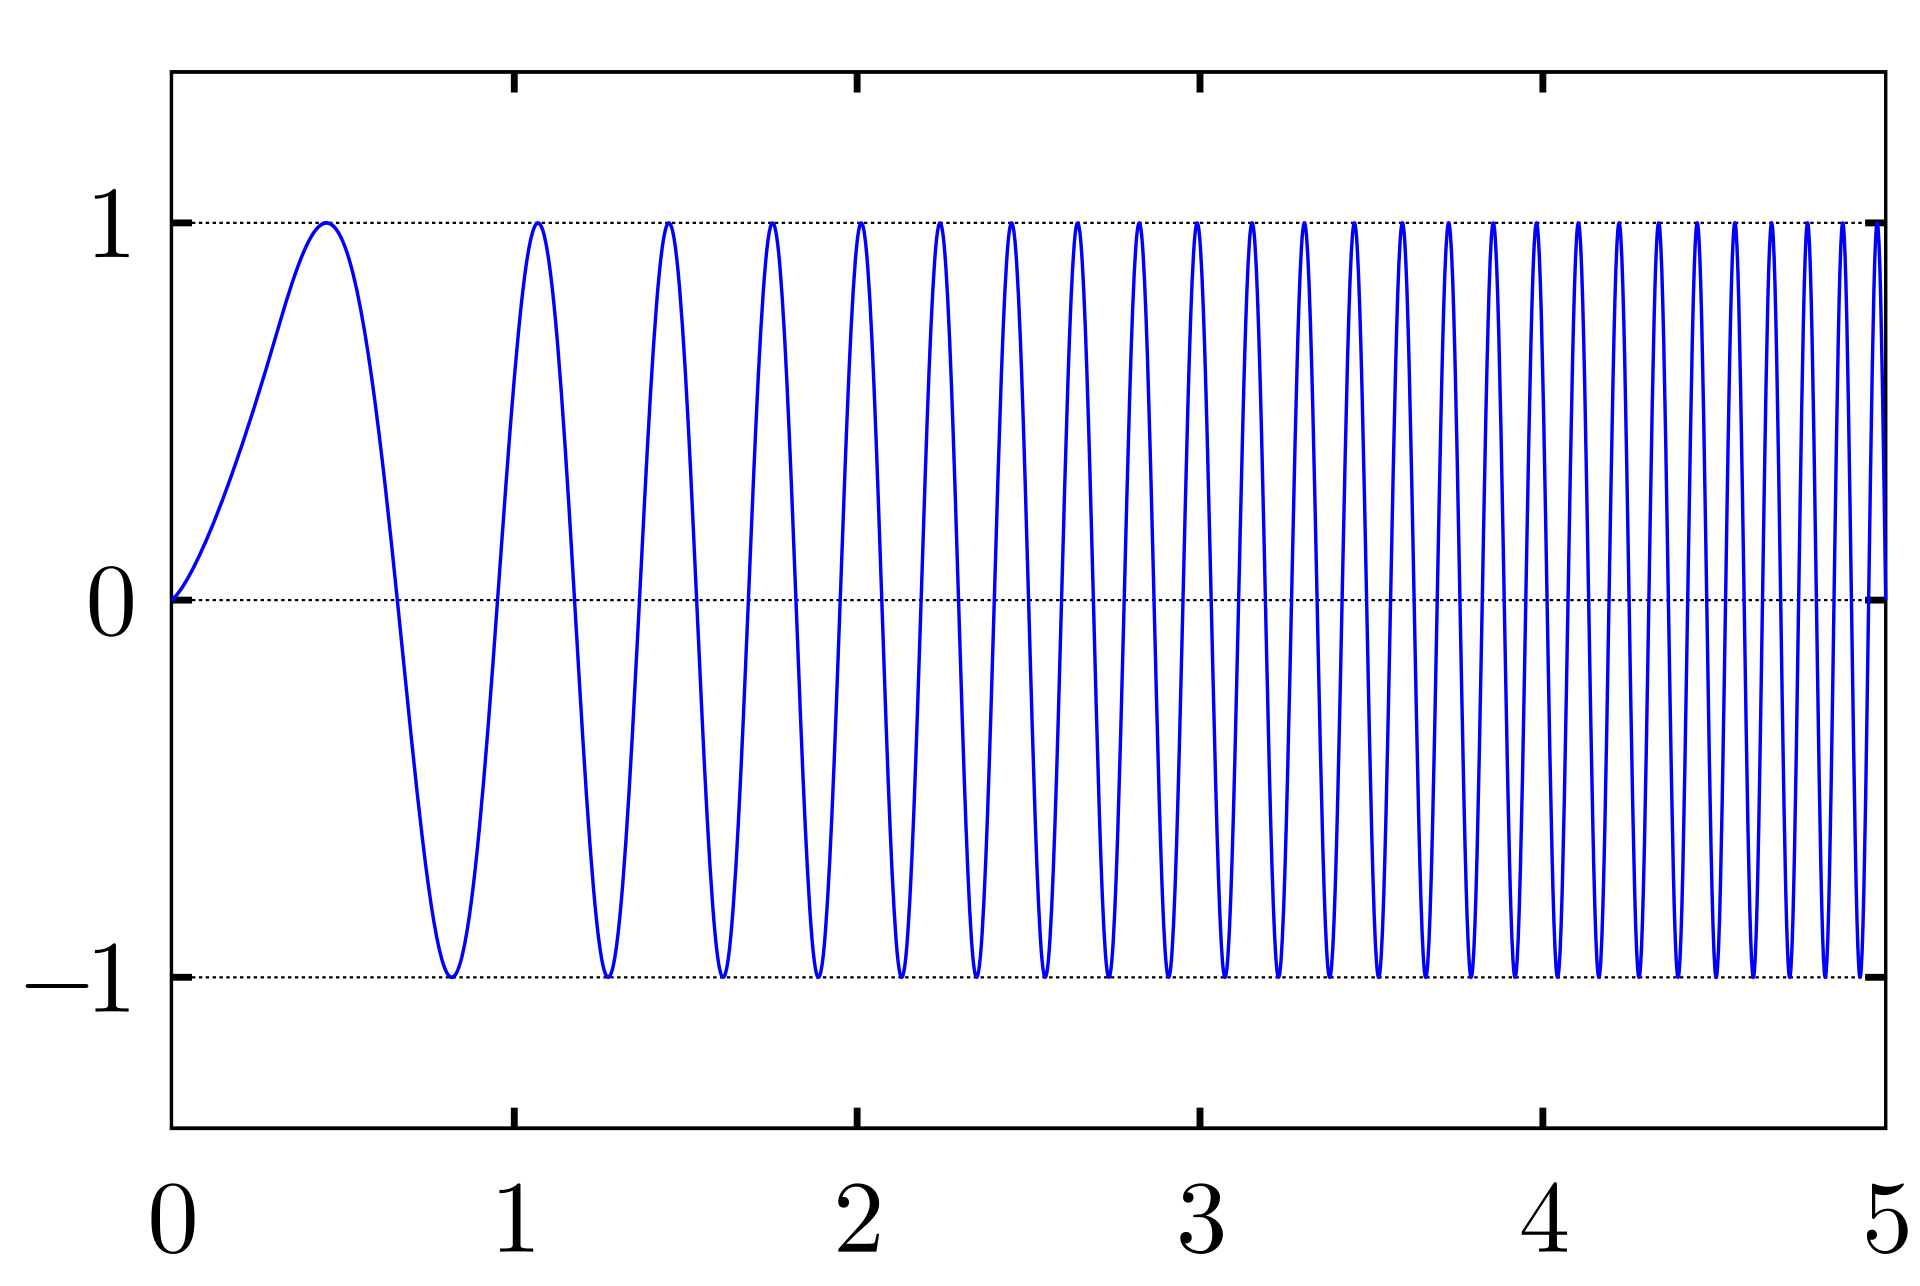
\includegraphics[width = \linewidth]{Linear-chirp.png}
                \caption{Modulación, ensanchado del espectro \citep{LoRaMod} }
                \label{fig:my_label}
            \end{subfigure}%
            \hfill
            \begin{subfigure}[t]{0.5\textwidth}
                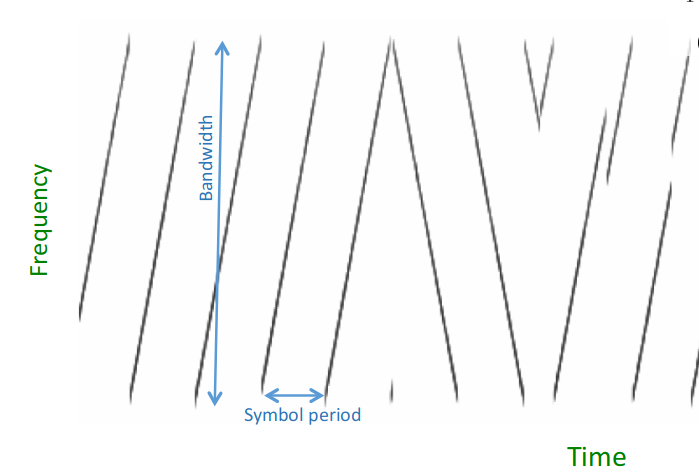
\includegraphics[width = \linewidth]{LoraModu.png}
                \caption{Caption}
                \label{fig:my_label}
            \end{subfigure}
    	
	\end{figure}

    Esta tecnología se caracteriza por su largo alcance, bajo consumo y bajo coste. También implementa tasas binaria variables, las cuales se  configuran utilizando factores de ensanchado ortogonales (SF o Spreading Factor por sus siglas en inglés), los cuales están en escala logarítmica e indican el número de chirps por símbolo de la modulación. La utilización de estos factores permiten elegir ente mejorar el alcance o la tasa binaria, utilizando un ancho de banda constante. 
    \paragraph{}
  	La relación entre la tasa binaria, el factor de ensanchado y el ancho de banda se define mediante la siguiente ecuación:

\begin{equation} \label{eq:rate}
	R_b = SF \times \frac{1}{[\frac{2^{SF}}{BW}]} (bit/sec)
\end{equation}
    
    Como podemos observar en la ecuación \ref{eq:rate}, al aumentar el valor de SF, disminuye la tasa binara de la modulación. Lo contrario pasa con el alcance máximo, el cual aumenta al aumentar el valor de SF. 
    
    \paragraph{}
    Definimos $SNR_{min}$ como la relación señal a ruido mínima que permite al receptor demodular la señal correctamente. Por otro lado, podemos definir la sensibilidad del receptor como:
    
    \begin{equation}
    	S_{re} = -174 + 10*{\log_{10} BW} + SNR_{min} + NF
    \end{equation}
    
    donde:
\begin{quote}
 \indent $BW$= Ancho de banda del canal \\
    \indent $SNR_{min}$ = Relación señal a ruido mínima\\
    \indent $NF$ = Figura de ruido del receptor (6bB)
\end{quote}   
   
    
    
    A modo de resumen, podemos ver en la tabla \ref{tab:sf} un ejemplo con los valores teóricos de una implementación con un ancho de banda de 125 KHz.
    
    
    \begin{table}[ht]
		\centering
    	\begin{tabular}{|c|c|c|c|} 
    
    		\hline
    		SF & $SNR_{min}$ (dB) & Sensibilidad (dBm) & Tasa binaria (Kbps) \\
    		\hline \hline
    		
    		7 &  -7.5  &  -125  & 6.83 \\
    		\hline 
    	
    		8 & -10 & -127 & 3.9 \\
    		\hline
    		9 & -12.5 & -130  & 2.19 \\
    		\hline
    		10 & -15 & -132 &  1.22 \\
    		\hline
    		11 & -17.5 & -135 & 0.671 \\
    		\hline
   			12 & -20 & -137 & 0.366 \\
    		\hline
        
		\end{tabular}
        \label{tab:sf}
   		\caption{Ejemplo teórico para un canal con 125 KHz de ancho de banda}
    \end{table}

    
    
	
    
    \subsection{Objetivos y motivaciones}
    
	Con la popularización de LoRa, se ha extendido la utilización de LoRaWAN como protocolo de comunicación. LoRaWAN es un protocolo de red , creado por \textit{LoRa Alliance}, que busca convertirse en un estándar.
\paragraph{}
El objetivo de este TFG será implementar un protocolo de comunicación, basado en LoRa, como alternativa a los ya existentes (LoRaWAN y SigFox). La principal motivación es el estudio de alternativas que impliquen un menor coste, eviten la utilización de hardware especifico y que, en futuras implementaciones, soporten un mayor número de arquitecturas de red.
\paragraph{}
Tras esto, haré una diseño hardware de nodos, enfocados a bajo consumo,
con transmisores LoRa. El objetivo será crear un nodo de tamaño reducido,
poco consumo y que pueda ser utilizado en múltiples aplicaciones. También
diseñaré placas con sensores que implementen estos nodos y que prueben su
funcionamiento.
\paragraph{}
Por último haré un estudio del funcionamiento del protocolo, alcance máximo
alcanzado y eficiencia energética de los nodos.
\paragraph{}
Cabe recalcar que la finalidad de este TFG no será crear un sistema que compita con LoRaWAN o con las redes que existen actualmente; lo que se busca, es aplicar los conocimientos sobre redes y sistemas de comunicación, adquiridos durante el grado, para implementar un protocolo de red y diseñar un hardware que lo soporte y probar el sistema final en un entorno real. 


    \subsection{Metodología }
    
	Con el fin de conseguir los objetivos planteados, se dividirá el trabajo en las siguientes fases:
	
	\begin{itemize}
		    \item Estudio de las tecnologías inalámbricas actuales y sus protocolos.
    	\item Estudio de LoRa y redes LPWAN
    	\item Diseño teórico del protocolo y su funcionamiento.
    	\item Elección de la plataforma hardware en la que se realizará el proyecto.
    	\item Implementación del protocolo.
    	\item Pruebas y depuración del protocolo mediante placas de desarrollo.
    	\item Diseño y fabricación del hardware.
    	\item Pruebas del sistema completo.
	\end{itemize}

